Strong scaling result is shown in the figure below.

\begin{figure}[htp]
\centering
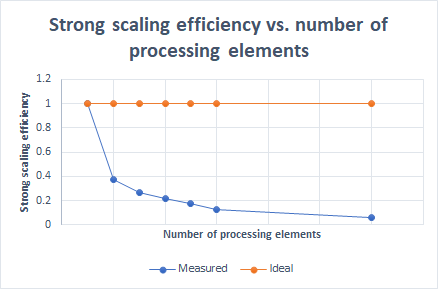
\includegraphics[width=\linewidth]{strong.png}
\caption{Strong scaling results}
\end{figure}

It can be observed that the strong scaling results are not very good but this is as expected. The overhead for the algorithm and communication increases as the number of processes increases and takes us to this result. It could be hard to reduce this part and we hadn't figure out how to do so.

And below is the weak scaling results.

\begin{figure}[htp]
\centering
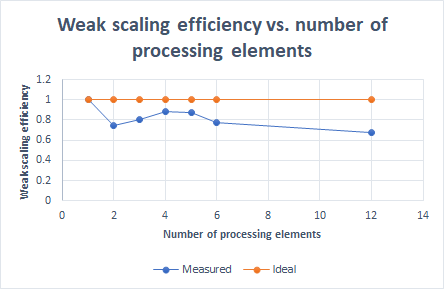
\includegraphics[width=\linewidth]{weak.png}
\caption{Weak scaling results}
\end{figure}

This result is better than the strong scaling result. In the sense that we didn't see significant drop in weak scaling efficiency as that in the strong scaling. Note that here is still a trend of dropping in the weak scaling efficiency.